\documentclass[12pt, a4paper]{article}

\usepackage{preamble}

\title{µC Compiler Design}
\author{Alexander Andersson \and Robin Eklind}
\date{\today}

% Document

\begin{document}

% === [ Front matter ] =========================================================

\pagenumbering{roman}

% --- [ Title page ] -----------------------------------------------------------

\maketitle

\clearpage

% --- [ Table of contents ] ----------------------------------------------------

\tableofcontents

\clearpage

% === [ Main matter ] ==========================================================

\pagenumbering{arabic}

% === [ Introduction ] =========================================================

\begin{quote}
	\textit{``Standing on the shoulders of dragons.''} \\ --- Anonymous
\end{quote}

\section{Introduction}
\label{sec:introduction}

% === [ Subsections ] ==========================================================

% --- [ Project Aim and Objectives ] -------------------------------------------

\subsection{Project Aim and Objectives}
\label{sec:intro_project_aim_and_objectives}

The aim of this project is to design and develop a compiler for the µC language, the grammar of which is specified in appendix \ref{app:informal_grammar_for_uc}.

To achieve this aim, the following objectives have been identified:

\begin{enumerate}
	\item \label{itm:obj_lexical_analysis} Construct a lexer for the µC language.
	\item \label{itm:obj_syntactic_analysis} Construct a parser for the µC language.
	\item \label{itm:obj_semantic_analysis} Implement a static semantic checker for the µC language.
	\item \label{itm:obj_intermediate_representation} Implement a library for interacting with LLVM IR or evaluate using an existing library.
	\item \label{itm:obj_ir_generation} Implement a translation from abstract syntax of the µC language to LLVM IR.
\end{enumerate}

% --- [ Deliverables ] ---------------------------------------------------------

\subsection{Deliverables}
\label{sec:intro_deliverables}

The source code and the report of this project have been released into the public domain\footnote{CC0 1.0 Universal: \url{https://creativecommons.org/publicdomain/zero/1.0/}} and are made available on GitHub at \url{https://github.com/mewmew/uc}.

The following document has been produced:

\begin{itemize}
	\item Project report; contained within the \texttt{report} directory of the source code repository.
\end{itemize}

And the following system artefacts have been developed:

\begin{itemize}
	\item Lexers (see objective~\ref{itm:obj_lexical_analysis}); contained within the \texttt{lexer} subdirectories of the source code repository.
	\item Parsers (see objective~\ref{itm:obj_syntactic_analysis}); contained within the \texttt{parser} subdirectories of the source code repository.
	\item Static semantic checker (see objective~\ref{itm:obj_semantic_analysis}).
	\item LLVM IR library (see objective~\ref{itm:obj_intermediate_representation}).
	\item IR code generator (see objective~\ref{itm:obj_ir_generation}); contained within the \texttt{irgen} directory of the source code repository.
\end{itemize}


% === [ Lexical Analysis ] =====================================================

\section{Lexical Analysis}
\label{sec:lexical_analysis}

\subsection{Notes}
\subsubsection{Extentions}
Using real C specification for following things, extending uC:
\begin{itemize}
	\item Add char Vertical tab (ASCII VT $11_{10}$) as extention whitespace
\end{itemize}

\subsubsection{Design decisions}
\begin{itemize}
	\item Return lexer to start of failing token to print error, continue lexing from following token.
	Sentiment: block comment errors, and potential later block token extention errors, will be easier to find by print out of start position of offending token
	\item The content in comments is not validated and may be of any charset, this is to allow for the common practice of using the current locale as character encoding in source file, and non-ASCII characters in comments.
\end{itemize}

\begin{verbatim}
'a'     // Ok
   ^ // Next token

'aa'x   // error
 ^ // Next token

'\a'    // error
 ^ // Next token

''              // error
 ^ // Next token

'\' // error
 ^ // Next token

"aa" // ok
    ^// Next token

"a\a"   //

"aa\" //

"aaEOF  // error


"\q/*" "\q*/"     // failing escape -> failing first quote,
 ^ // Next tokken // starting and ending block comment,
                  // starting new eventually failing quote

\end{verbatim}
foo \cite{lexical_scanning_in_go}

% === [ Syntactic Analysis ] ===================================================

\section{Syntactic Analysis}
\label{sec:syntactic_analysis}

foo

\subsection{uC Type Representations}
\label{app:semantic/types_doc}

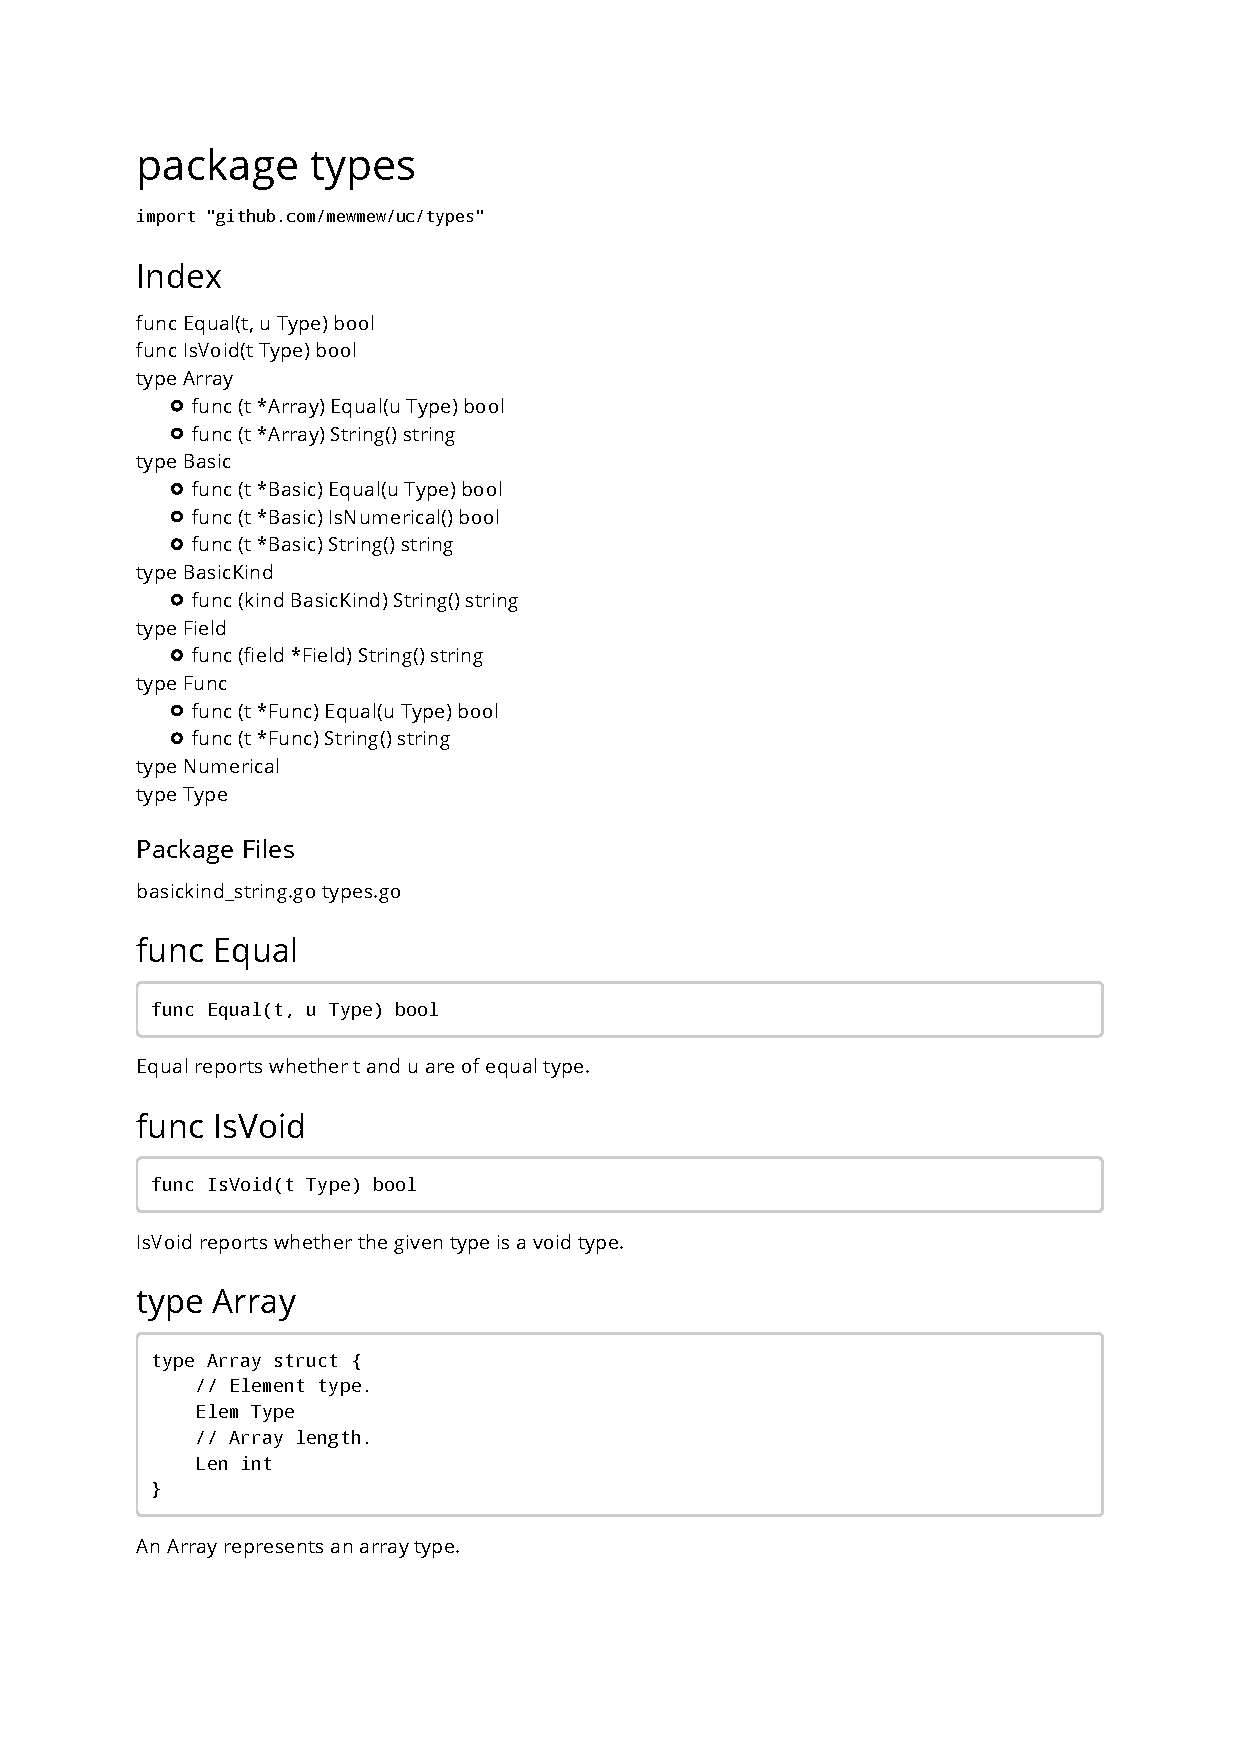
\includepdf[pages=-]{inc/sections/4_semantic_analysis/types_doc.pdf}

\clearpage

\subsection{Semantic Analysis Test Cases}
\label{app:semantic/testcases}

\subsubsection{Correct Test Cases}
\label{app:semantic/correct}

\input{inc/usem/quiet/semantic/listing.tex}
\input{inc/usem/noisy/advanced/listing.tex}

\clearpage % TODO: Find better solution.

\subsubsection{Incorrect Test Cases}
\label{app:semantic/incorrect}

\input{inc/usem/incorrect/semantic/listing.tex}

\subsubsection{Extra Test Cases}
\label{app:semantic/extra}

\input{inc/usem/extra/semantic/listing.tex}

%% === [ Intermediate Representation ] ==========================================

\section{Intermediate Representation}
\label{sec:intermediate_representation}

\subsection{Design Decisions}

The design of the parser has been guided by the KISS philosophy, were simplicity rule supreme.

\subsubsection{Unified Types}

To simplify the design of the syntactic analysis phase, types have been given a unified representation in the grammar. As a consequence of this design decision, certain invalid type declarations are syntactically valid, such as \texttt{void x[10];}. To facilitate separation of concern between components of the compiler, proper type checking has initially been postponed to the semantic analysis phase\footnote{Postpone type checking to the semantic analysis phase: \url{https://github.com/mewmew/uc/issues/33}}.

\subsubsection{Unified Declarations}

To further simplify the grammar, variable and function declarations have been given a unified representation in the grammar\footnote{Evaluate merging TopLevelDecl with Decl to simplify grammar: \url{https://github.com/mewmew/uc/issues/38}}. As a consequence of this design decision, nested function declarations are syntactically valid (see listing \ref{fig:nested_func_decl}), but not necessarily semantically valid.

\begin{lstlisting}[language=C,style=c,caption={\label{fig:nested_func_decl}Nested function declarations.}]
int add(int a, int b) {
	// Nested function declarations are syntactically valid.
	int nested(void) {
		return a + b;
	}
	return nested();
}
\end{lstlisting}

The static checker of the semantic analysis phase will ensure that functions contain no nested function declarations, unless the relevant GNU extension has been enabled\footnote{Add support for nested functions (GNU extension): \url{https://github.com/mewmew/uc/issues/43}}.

\subsubsection{Ignored Comments}

As comments may appear between any two tokens of the input stream, the production rules of the grammar would be significantly more complex if forced to deal with the possible occurrences of comments. For this reason, comments have been filtered from the token stream before the syntactic analysis stage. This design decision simplifies the grammar, but prevents the parser from being used for the development of source code rewriting and documentation generation tools, both of which require access to comments\footnote{Production rules made more complex by comment tokens: \url{https://github.com/mewmew/uc/issues/30}}.

\subsection{Implementation}

The parser was generated using Gocc from a BNF grammar of the uC language, the listing of which is presented in Appendix~\ref{app:parser/gocc}. The precedence and associativity of binary operators have been cross-referenced against §6.5 of the C11 specification \cite{c11_spec}.

\subsubsection{Precedence of Binary Operators}

Precedence of binary operators is implemented in the BNF grammar through a tree-like structure of production rules (actually a graph structure, as nodes may be self-referential and refer to parental nodes), having operators with lower precedence near the root of the tree and operators with higher precedence near the leafs of the tree.

An example of the production rules used to assign a higher precedence to multiplicative operators than additive operators is presented in listing \ref{lst:precedence}.

\begin{lstlisting}[language=go,style=go,caption={\label{lst:precedence}Precedence of binary expressions.}]
// Left-associative binary expressions with precedence 12.
//
//    12L: + -
Expr12L
	: Expr13L
	| Expr12L "+" Expr13L
	| Expr12L "-" Expr13L
;

// Left-associative binary expressions with precedence 13.
//
//    13L: * /
Expr13L
	: Expr14
	| Expr13L "*" Expr14
	| Expr13L "/" Expr14
;
\end{lstlisting}

\subsubsection{Associativity of Binary Operators}

The implementation of left- and right-associativity of binary operators relies on the same tree-like structure as the implementation of operator precedence. The non-terminal node on the right side of a right-associative binary operator (e.g. \texttt{Expr2R} of \texttt{Expr5L ``='' Expr2R}) is self-referential, while the non-terminal node on the left side of the operator (e.g. \texttt{Expr5L} of \texttt{Expr5L ``='' Expr2R}) refers to a node closer to the leaf nodes of the tree. Left-associativity is defined analogously, with a self-referential left side node.

An example of the production rules used to define right-associativity to assignment operators and left-associativity to logical AND operators is presented in listing \ref{lst:associativity}.

\begin{lstlisting}[language=go,style=go,caption={\label{lst:associativity}Associativity of binary expressions.}]
// Right-associative binary expressions with precedence 2.
//
//    2R: =
Expr2R
	: Expr5L
	// Right-associative.
	| Expr5L "=" Expr2R
;

// Left-associative binary expressions with precedence 5.
//
//    5L: &&
Expr5L
	: Expr9L
	| Expr5L "&&" Expr9L
;
\end{lstlisting}

\subsubsection{Syntax Tree Representation}

% You should also describe the representation of syntax trees and list the different kinds of nodes.

% TODO: Add syntax tree representation.

foo

\subsubsection{Dangling Else}

The dangling else problem is the canonical example of a shift-reduce conflict for LR grammars, and it is present in the µC grammar presented in Appendix~\ref{app:parser/gocc}. When generating a parser from this grammar, Gocc was capable of identifying the shift-reduce conflict introduce by the dangling else problem. Furthermore, Gocc provided an option for automatically resolving shift-reduce conflicts\footnote{Dangling else: \url{https://github.com/mewmew/uc/issues/31}} by applying \textit{maximum-munch}, as further described by the following extract from the Gocc user guide \cite{gocc_user_guide}.

\begin{quote}
	\begin{lstlisting}[language=go,style=go,caption={Grammar with shift-reduce conflict.}]
	Stmt
		: "if" Expr "then" Stmt
		| "if" Expr "then" Stmt "else" Stmt
	;
	\end{lstlisting}

	\textit{``When automatic LR(1) conflict resolution is selected by the -a option, gocc resolves this conflict in the same way as specified in the C language specification: by shifting and parsing the longest valid production (maximal-munch). This means recognising the else-statement as part of the second if.''}
\end{quote}

\subsection{Validation}

\subsubsection{Correct Test Cases}

For listings, see Appendix~\ref{app:semantic/correct}: \nameref{app:semantic/correct}:
\input{inc/usem/quiet/semantic/listref.tex}
\input{inc/usem/noisy/advanced/listref.tex}

\subsubsection{Incorrect Test Cases}

For listings, see Appendix~\ref{app:semantic/incorrect}: \nameref{app:semantic/incorrect}:
\input{inc/usem/incorrect/semantic/listref.tex}

\subsubsection{Extra Test Cases}

For listings, see Appendix~\ref{app:semantic/extra}: \nameref{app:semantic/extra}:
\input{inc/usem/extra/semantic/listref.tex}

 % skipped for now
% === [ IR Generation ] ========================================================

\section{IR Generation}
\label{sec:ir_generation}

One of the first decisions made when deciding to implement a compiler for the uC programming language was to target LLVM IR, rather than MIPS, as this would allow for native code generation to a wide variety of platforms, such as x86 and ARM.

A large amount of preparatory work was made before developing the IR generation phase of the compiler, in particular a library for LLVM IR was developed which implements support for parsing LLVM IR assembly files and provides an in-memory representation of LLVM IR which is capable of pretty-printing itself to LLVM IR assembly code. The design of the LLVM IR generator of the compiler has guided the design of the API for the LLVM IR library. The full API is too vast to cover here, but its documentation has been available online.

\begin{itemize}
	\item \url{https://godoc.org/github.com/llir/llvm/ir}
	\item \url{https://godoc.org/github.com/llir/llvm/ir/constant}
	\item \url{https://godoc.org/github.com/llir/llvm/ir/instruction}
	\item \url{https://godoc.org/github.com/llir/llvm/ir/types}
	\item \url{https://godoc.org/github.com/llir/llvm/ir/value}
\end{itemize}

Before diving into the design details of the IR generation phase of the compiler, a brief installation and usage introduction of the compiler is presented in section \ref{sec:installation_and_usage}, so that the interested reader may evaluate the compiler themselves on real world uC programs.

% === [ Subsections ] ==========================================================

\subsection{Installation and Usage}
\label{sec:installation_and_usage}

This section provides a brief introduction to the installation procedure and usage of the \texttt{uclang} compiler.

\subsubsection{Installation}

As a prerequisite, install a compiler for the Go programming language. See \url{https://golang.org/doc/install} for installation instructions. Make sure to configure the \texttt{GOPATH} environment variable, to specify a directory for the workspace.

Once Go has been installed and a \texttt{GOPATH} workspace has been configured, it should be possible to retrieve the source code of remote repositories and install the tools and packages contained within, using the \texttt{go} tool with the \texttt{get} command.

To generate lexers and parsers for uC source code and LLVM IR assembly the Gocc tool is used. To install Gocc, invoke the following command.

\begin{verbatim}
$ go get github.com/goccmack/gocc
\end{verbatim}

Once compiled, the \texttt{gocc} tool is placed within the \verb+$GOPATH/bin+ directory. Make sure to add this directory to the \texttt{PATH} environment variable, for subsequent \texttt{Makefile}s to work.

To simplify the generation of test cases, a regular expression search and replace tool called \texttt{sar} has been used. To download \texttt{sar}, invoke the following command.

\begin{verbatim}
$ go get github.com/mewkiz/cmd/sar
\end{verbatim}

With the prerequisites out of the way, lets take a look at how to download and install the \texttt{uclang} compiler itself. To download the compiler, and all other tools and libraries related to it, invoke the following command. You may safely ignore the warning that the \texttt{uc} directory contains no buildable Go source files.

\begin{verbatim}
$ go get -d github.com/mewmew/uc
\end{verbatim}

Now we are ready to generate the lexer and parser for uC. Traverse into the \texttt{gocc} directory of the \texttt{uc} repository and invoke \texttt{make}, i.e. invoke the following commands.

\begin{verbatim}
$ cd $GOPATH/src/github.com/mewmew/uc/gocc
$ make
\end{verbatim}

After generating the uC lexer and parser, invoke the following command to install the lexer tool, parser tool, semantic analysis tool and the uC compiler tool,

\begin{verbatim}
$ go get github.com/mewmew/uc/...
\end{verbatim}

Now, the lexer tool (\texttt{ulex}), parser tool (\texttt{uparse}), semantic analysis tool (\texttt{usem}) and the uC compiler (\texttt{uclang}) should have been compiled and installed into the \verb+$GOPATH/bin+ directory.

\subsubsection{Usage}

For usage instructions, invoke the respective commands with the \verb+-help+ flag, or refer to the online documentation.

\begin{itemize}
	\item \texttt{ulex}: \url{https://godoc.org/github.com/mewmew/uc/cmd/ulex}
	\item \texttt{uparse}: \url{https://godoc.org/github.com/mewmew/uc/cmd/uparse}
	\item \texttt{usem}: \url{https://godoc.org/github.com/mewmew/uc/cmd/usem}
	\item \texttt{uclang}: \url{https://godoc.org/github.com/mewmew/uc/cmd/uclang}
\end{itemize}

For the remainder of this section, the usage of the uC compiler \texttt{uclang} is explored and illustrated through examples.

To compile a uC source file (e.g. \texttt{foo.c}) and emit the corresponding LLVM IR assembly code to standard output, invoke the following command.

\begin{verbatim}
$ uclang foo.c
\end{verbatim}

To compile a uC source file (e.g. \texttt{foo.c}) and emit the corresponding LLVM IR assembly code to a given output file (e.g. \texttt{foo.ll}), invoke the following command.

\begin{verbatim}
$ uclang -o foo.ll foo.c
\end{verbatim}

A slightly modified version of the runtime library containing the \texttt{getint} and \texttt{putstring} functions is located at \texttt{testdata/uc.c}, and the corresponding LLVM IR assembly (compiled with Clang, since \texttt{uclang} has yet to support string literals) is located at \texttt{testdata/uc.ll}.

Using the standard \texttt{llvm-link} tool from the LLVM compiler framework, two or more LLVM IR assembly files may be linked together, or merged. This provides a useful way of linking the runtime library into compiled programs which makes use of the \texttt{getint} or \texttt{putstring} functions, such as \texttt{testdata/noisy/advanced/eval.c}. On a side node, a missing return statement has been added to the \texttt{eval} function of the \texttt{eval.c} test case source code, as the static semantic analysis checker would otherwise have terminated the compilation of the otherwise interesting test program.

To compile the \texttt{eval} test program into LLVM IR assembly, invoke the following commands.

\begin{verbatim}
$ cd $GOPATH/src/github.com/mewmew/uc
$ uclang -o out.ll testdata/noisy/advanced/eval.c
$ llvm-link -o eval.ll out.ll testdata/uc.ll
\end{verbatim}

The standard \texttt{lli} LLVM IR interpretor may then be used to invoke the resulting LLVM IR assembly file as such.

\begin{verbatim}
$ lli eval.ll
\end{verbatim}

Another option is to compile the LLVM IR assembly file to a host native binary application, by invoking the following standard command from the LLVM compiler framework.

\begin{verbatim}
$ llc -o eval.S eval.ll
$ as -o eval.o eval.S
$ ld -o eval -dynamic-linker /usr/lib/ld-linux-x86-64.so.2 /usr/lib/crt1.o
/usr/lib/crti.o /usr/lib/crtn.o eval.o -lc
\end{verbatim}

While it is possible to successfully compile and link LLVM IR assembly files using the \texttt{llc}, \texttt{as} and \texttt{ld} commands, simply invoking Clang to accomplish the same task if often far easier.

\begin{verbatim}
$ clang -o eval eval.ll
\end{verbatim}

\subsubsection{Test Cases}

To run the test cases, simply invoke the \texttt{go} tool with the \texttt{test} command and the Go import path of the package to test.

To test all packages invoke \texttt{go test github.com/mewmew/uc/...} or run the following commands.

\begin{verbatim}
$ go test github.com/mewmew/uc/token
$ go test github.com/mewmew/uc/gocc/lexer
$ go test github.com/mewmew/uc/hand/lexer
$ go test github.com/mewmew/uc/gocc/scanner
$ go test github.com/mewmew/uc/gocc/parser
$ go test github.com/mewmew/uc/sem
$ go test github.com/mewmew/uc/irgen
\end{verbatim}

\subsection{Design Decisions}

The \texttt{uclang} compiler is designed to output LLVM IR assembly which is almost identical to the LLVM IR assembly generated by Clang for a given µC program. The main benefit of this decision is to facilitate validation, as further described in section \ref{sec:irgen_validation}.

\subsubsection{Local Identifiers}

An explicit aim of LLVM IR is to remove the requirement of using other intermediate representations within the compiler middle-end \cite{osa_llvm}. To achieve this aim, the IR must be capable of supporting a wide range of optimization passes, while remaining platform independent. This is accomplished with a platform independent RISC assembly language, similar to MIPS but with support for an infinite amount of registers; as is common for Register Transfer Languages. Local IDs are assigned to keep track of these registers, and within LLVM IR, there exist a notion of unnamed local identifiers, where the ID (an integer) is inferred using a function specific counter starting from 0. The first unnamed local ID is assigned 0, the second 1, and so on, in any given function.

A core concept within LLVM IR is the notion of a \textit{value}, which is the result of a computation that may be used by other \textit{values}. Building upon this idea, an LLVM IR library has been developed which keeps track of registers, not by their explicit names, but by references to the computation which produced the register, often an arithmetic instruction. As all the key concepts within LLVM IR as represented as values, namely global variables, functions, function parameters, basic blocks, and registers assigned from instruction computations, the LLVM IR library does not keep track of names, but rather references to values, when building instructions which refer to the computed values of other instructions. This is a powerful concept, as it allows for the generation of LLVM IR, without the need to explicitly specify the names of registers. The main advantage of this is that the LLVM IR library may take the responsibility of generating consecutive sequences of local IDs, thus freeing users of the library from having to keep track of the function specific counter.

\subsubsection{Control Flow}

The control flow of a µC program is determined by the use of \texttt{if}, \texttt{else}, \texttt{while} and \texttt{return} statements and calls to functions. In our code generation, we translate the first constructs to llvm basic blocks with conditional jumping with the calls and returns staying essentially the same.

%\subsubsection{Implicit Conversion}
%TODO: alex

% Skipping this section fow now.

%\subsection{Implementation}

%\subsubsection{Control Flow}
%TODO: alex

%\subsubsection{Implicit Conversion}
%TODO: alex

\subsection{Validation}
\label{sec:irgen_validation}

As the LLVM IR generated by the \texttt{uclang} compiler has been intentionally kept very close to the LLVM IR generated by Clang for a given uC program, testing the implementation of the IR generator becomes almost trivial. The test cases simply use Clang to generate LLVM IR from input C source files, each covering a specific language features, such as while loops or array index expressions. Since Clang outputs a lot of metadata, which is not strictly related to the semantics of the program, a post-processing script has been developed which removes any unnecessary metadata, function attributes, comments or other LLVM IR language constructs which are not required to run the test programs. The post-processed LLVM IR assembly output from Clang is then compared against the LLVM IR generated by the \texttt{uclang} IR generation algorithm, and the test case passes if the outputs are identical and it fails otherwise.

To the best of our knowledge, the LLVM IR generated by \texttt{uclang} should be valid for all possible uC programs, with one exception array index expressions and array references in functions taking arrays as input parameters. That being said, we have discovered a wide range of issues with the generation algorithm while developing it, and have added specific test cases to ensure that fixed bugs are not reintroduced at a later point of development.

To run the test cases of the IR generation library, invoke the following command.

\begin{verbatim}
$ go test github.com/mewmew/uc/irgen
\end{verbatim}

The input source files used to validate the IR generation algorithm may be located in the \texttt{testdata/extra/irgen} directory of the \texttt{uc} repository.

\subsubsection{Example Output}

The listing example illustrates the LLVM IR output (see listing \ref{lst:r06.ll}) generated by \texttt{uclang} when compiling the Fibonacci test case \texttt{testdata/quiet/rtl/r06.c} (see listing \ref{lst:quiet/rtl/r06.c}). Note, the \texttt{r06.c} source file has been slightly modified, to commend out the preprocessing include directive and to include a return statement from main, returning the value calculated by the \texttt{fib} function as a status code from the progam.

\lstinputlisting[style=c,language=C,caption=quiet/rtl/r06.c,label=lst:quiet/rtl/r06.c]{inc/sections/6_ir_generation/r06.c}

\lstinputlisting[style=c,language=llvm,caption=r06.ll,label=lst:r06.ll]{inc/sections/6_ir_generation/r06.ll}

To compile test \texttt{r06.c} source file and run the resulting LLVM IR assembly code, invoke the following commands.

\begin{verbatim}
$ uclang -o r06.ll r06.c
$ lli r06.ll ; echo $?
\end{verbatim}

Executing the above command will print the status code \texttt{120} to standard output, thus confirming that the fifth Fibonacci number was indeed calculated correctly.

%\subsubsection{Correct RTL Test Cases}

%For listings, see Appendix~\ref{app:irgen/correct}: \nameref{app:irgen/correct}:
%\input{inc/uclang/quiet/rtl/listref.tex}

%\subsubsection{Extra Test Cases}

%For listings, see Appendix~\ref{app:irgen/extra}: \nameref{app:irgen/extra}:
%\input{inc/uclang/noisy/advanced/listref.tex}
%\input{inc/uclang/extra/irgen/listref.tex}


%% === [ Conclusion ] ===========================================================

\section{Conclusion}
\label{sec:conclusion}

This section concludes the project report with subjective reflections from the project authors. For the remainder of this section we will switch to a first person narrative.

TODO: what have been easier or hardet to do? robin

TODO: future work

% === [ Subsections ] ==========================================================

% --- [ Project Summary ] ------------------------------------------------------

\subsection{Project Summary}
\label{sec:project_summary}

foo

% --- [ Project Future ] -------------------------------------------------------

\subsection{Project Future}
\label{sec:project_future}

Since a very early stage of development, we were both discussing where we may wish to take this project in the future and how we may wish to continue developing it. The obvious aims for the future would be to extend the supported language constructs of C. Prior to this work, we intend to spend some time cleaning up the code base, reviewing past design decisions and fixing issues caused by time constraints (such as the IR generation of array index expressions, etc).

Supplementary future plans for the project is to continue developing the LLVM IR library, and make it available for general use by other Go projects which may wish to interact with LLVM IR. The library is already being used by a decompiler project to generate control flow graphs from LLVM IR.

% --- [ Final Thoughts ] -------------------------------------------------------

\subsection{Final Thoughts}
\label{sec:final_thoughts}

It is difficult to pinpoint exactly what it is about compilers and compiler development that is so captivating. Gaining a deeper understanding of programming languages by looking under the hood of the low-level abstractions provides a refreshing insight into the conceptual building blocks which guide our thoughts and creative processes when developing software.

To conclude, it does feel like a right of passage to develop a C compiler on your own. We feel honoured to have been given this opportunity of doing so, and would recommend anyone interested to give it a shot. But be careful, compiler development is addictive!

 % skipped for now.

% === [ Back matter ] ==========================================================

% --- [ References ] -----------------------------------------------------------

\bibliography{references}

% --- [ Appendices ] -----------------------------------------------------------

% === [ Appendices ] ===========================================================

\appendix
\setcounter{secnumdepth}{0}
\section{Appendices}
\setcounter{secnumdepth}{3}
\renewcommand{\thesubsection}{\Alph{subsection}}

% --- [ Informal grammar for µC ] ----------------------------------------------

\subsection{Informal grammar for µC}
\label{app:informal_grammar_for_uc}

This is an informal context-free grammar for uC (included without modification from \url{https://www.it.uu.se/katalog/aleji304/CompilersProject/uc.html}):

\begin{itemize}
	\item The start symbol is \texttt{program}.
	\item Keywords and special symbols are written within double-quotes.
	\item \texttt{/empty/} denotes the empty string.
	\item \texttt{intconst} and \texttt{ident} denote classes of lexical elements.
	\item Associativity and precedence for expression operators is not expressed.
	\item The grammar has not been adjusted to fit any particular parsing method.
\end{itemize}

\begin{verbatim}
program         ::= topdec_list
topdec_list     ::= /empty/ | topdec topdec_list
topdec          ::= vardec ";"
                  | funtype ident "(" formals ")" funbody
vardec          ::= scalardec | arraydec
scalardec       ::= typename ident
arraydec        ::= typename ident "[" intconst "]"
typename        ::= "int" | "char"
funtype         ::= typename | "void"
funbody         ::= "{" locals stmts "}" | ";"
formals         ::= "void" | formal_list
formal_list     ::= formaldec | formaldec "," formal_list
formaldec       ::= scalardec | typename ident "[" "]"
locals          ::= /empty/ | vardec ";" locals
stmts           ::= /empty/ | stmt stmts
stmt            ::= expr ";"
                  | "return" expr ";" | "return" ";"
                  | "while" condition stmt
                  | "if" condition stmt else_part
                  | "{" stmts "}"
                  | ";"
else_part       ::= /empty/ | "else" stmt
condition       ::= "(" expr ")"
expr            ::= intconst
                  | ident | ident "[" expr "]"
                  | unop expr
                  | expr binop expr
                  | ident "(" actuals ")"
                  | "(" expr ")"
unop            ::= "-" | "!"
binop           ::= "+" | "-" | "*" | "/"
                  | "<" | ">" | "<=" | ">=" | "!=" | "=="
                  | "&&"
                  | "="
actuals         ::= /empty/ | expr_list
expr_list       ::= expr | expr "," expr_list
\end{verbatim}

\clearpage
% === [ Lexical Analysis ] =====================================================

\section{Lexical Analysis}
\label{sec:lexical_analysis}

\subsection{Notes}
\subsubsection{Extentions}
Using real C specification for following things, extending uC:
\begin{itemize}
	\item Add char Vertical tab (ASCII VT $11_{10}$) as extention whitespace
\end{itemize}

\subsubsection{Design decisions}
\begin{itemize}
	\item Return lexer to start of failing token to print error, continue lexing from following token.
	Sentiment: block comment errors, and potential later block token extention errors, will be easier to find by print out of start position of offending token
	\item The content in comments is not validated and may be of any charset, this is to allow for the common practice of using the current locale as character encoding in source file, and non-ASCII characters in comments.
\end{itemize}

\begin{verbatim}
'a'     // Ok
   ^ // Next token

'aa'x   // error
 ^ // Next token

'\a'    // error
 ^ // Next token

''              // error
 ^ // Next token

'\' // error
 ^ // Next token

"aa" // ok
    ^// Next token

"a\a"   //

"aa\" //

"aaEOF  // error


"\q/*" "\q*/"     // failing escape -> failing first quote,
 ^ // Next tokken // starting and ending block comment,
                  // starting new eventually failing quote

\end{verbatim}
foo \cite{lexical_scanning_in_go}

\clearpage
% === [ Syntactic Analysis ] ===================================================

\section{Syntactic Analysis}
\label{sec:syntactic_analysis}

foo

\clearpage
\subsection{uC Type Representations}
\label{app:semantic/types_doc}

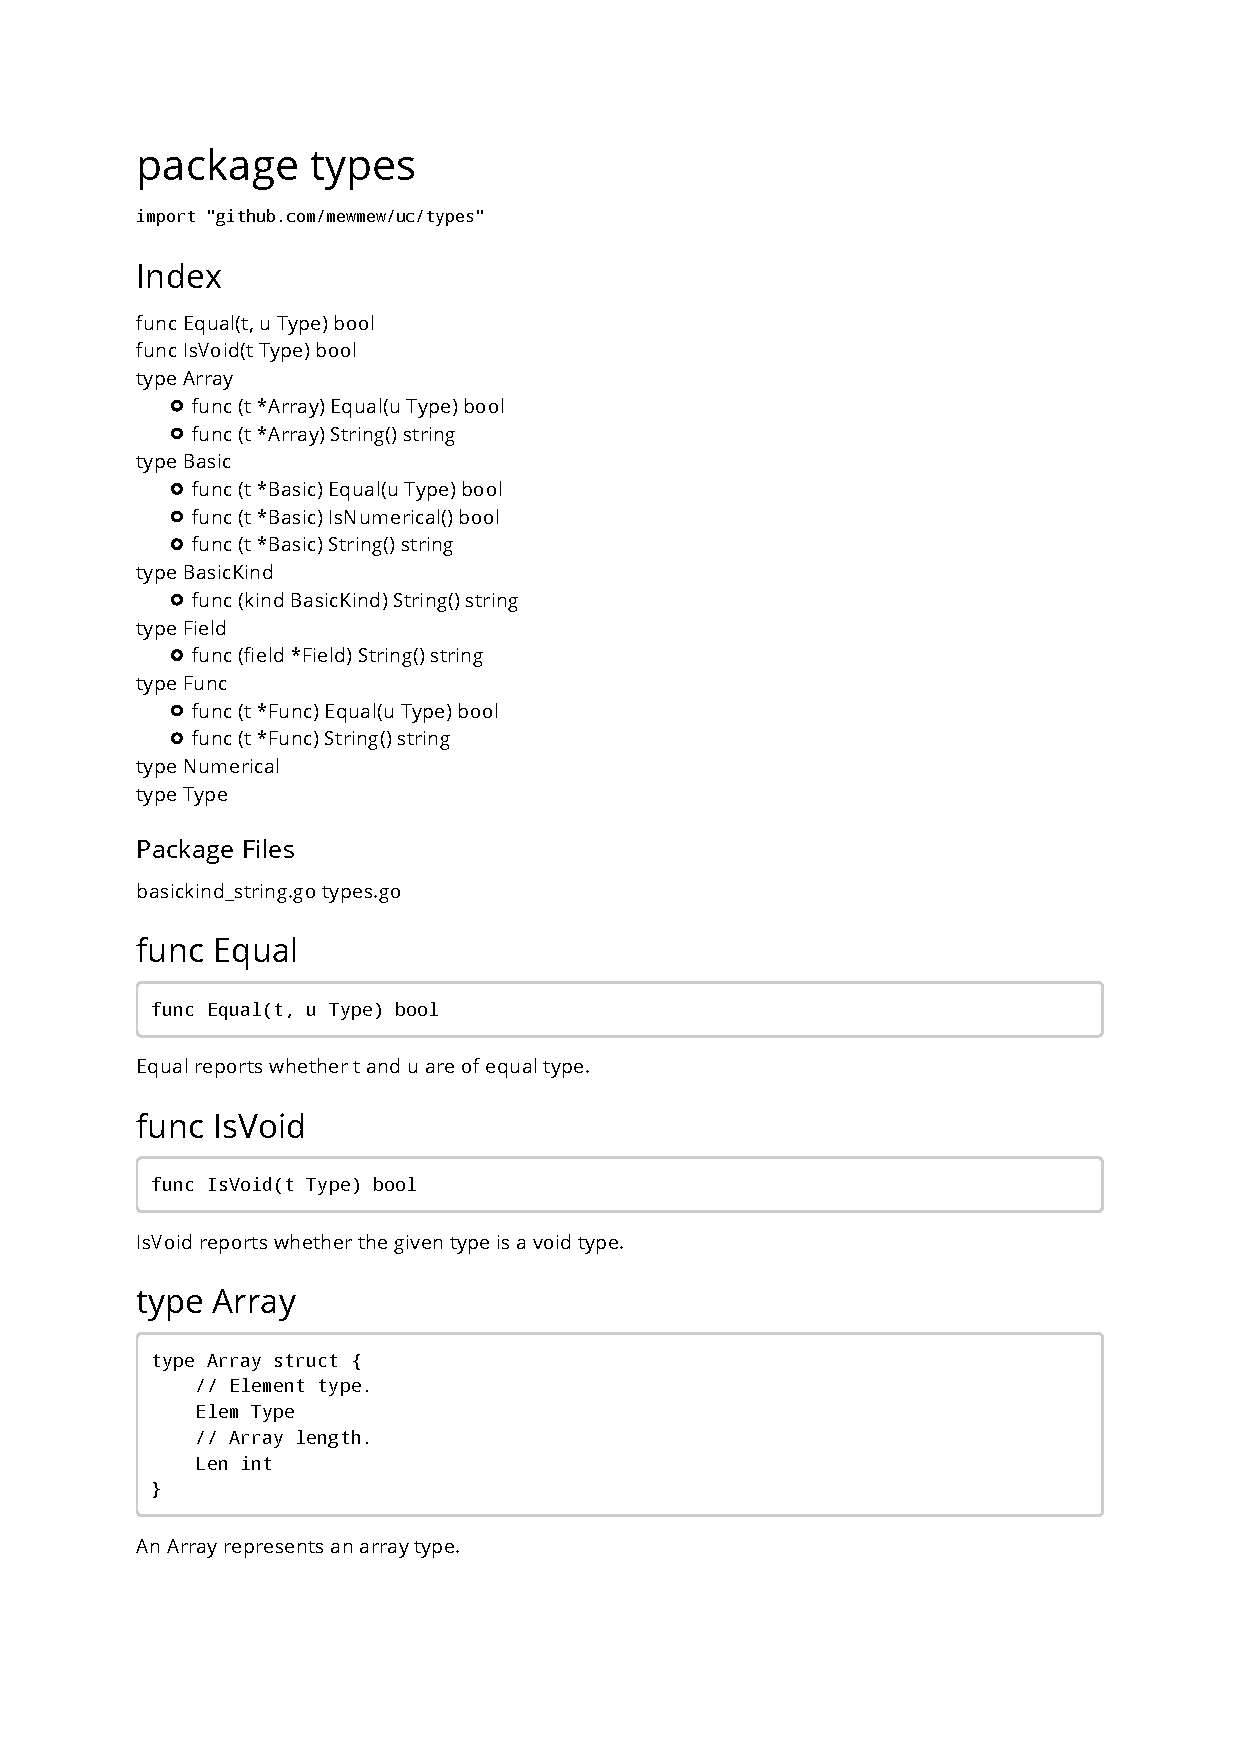
\includepdf[pages=-]{inc/sections/4_semantic_analysis/types_doc.pdf}

\clearpage

\subsection{Semantic Analysis Test Cases}
\label{app:semantic/testcases}

\subsubsection{Correct Test Cases}
\label{app:semantic/correct}

\input{inc/usem/quiet/semantic/listing.tex}
\input{inc/usem/noisy/advanced/listing.tex}

\clearpage % TODO: Find better solution.

\subsubsection{Incorrect Test Cases}
\label{app:semantic/incorrect}

\input{inc/usem/incorrect/semantic/listing.tex}

\subsubsection{Extra Test Cases}
\label{app:semantic/extra}

\input{inc/usem/extra/semantic/listing.tex}



\end{document}
